\documentclass[12pt]{article}\usepackage[]{graphicx}\usepackage[]{color}
%% maxwidth is the original width if it is less than linewidth
%% otherwise use linewidth (to make sure the graphics do not exceed the margin)
\makeatletter
\def\maxwidth{ %
  \ifdim\Gin@nat@width>\linewidth
    \linewidth
  \else
    \Gin@nat@width
  \fi
}
\makeatother

\definecolor{fgcolor}{rgb}{0.345, 0.345, 0.345}
\newcommand{\hlnum}[1]{\textcolor[rgb]{0.686,0.059,0.569}{#1}}%
\newcommand{\hlstr}[1]{\textcolor[rgb]{0.192,0.494,0.8}{#1}}%
\newcommand{\hlcom}[1]{\textcolor[rgb]{0.678,0.584,0.686}{\textit{#1}}}%
\newcommand{\hlopt}[1]{\textcolor[rgb]{0,0,0}{#1}}%
\newcommand{\hlstd}[1]{\textcolor[rgb]{0.345,0.345,0.345}{#1}}%
\newcommand{\hlkwa}[1]{\textcolor[rgb]{0.161,0.373,0.58}{\textbf{#1}}}%
\newcommand{\hlkwb}[1]{\textcolor[rgb]{0.69,0.353,0.396}{#1}}%
\newcommand{\hlkwc}[1]{\textcolor[rgb]{0.333,0.667,0.333}{#1}}%
\newcommand{\hlkwd}[1]{\textcolor[rgb]{0.737,0.353,0.396}{\textbf{#1}}}%

\usepackage{framed}
\makeatletter
\newenvironment{kframe}{%
 \def\at@end@of@kframe{}%
 \ifinner\ifhmode%
  \def\at@end@of@kframe{\end{minipage}}%
  \begin{minipage}{\columnwidth}%
 \fi\fi%
 \def\FrameCommand##1{\hskip\@totalleftmargin \hskip-\fboxsep
 \colorbox{shadecolor}{##1}\hskip-\fboxsep
     % There is no \\@totalrightmargin, so:
     \hskip-\linewidth \hskip-\@totalleftmargin \hskip\columnwidth}%
 \MakeFramed {\advance\hsize-\width
   \@totalleftmargin\z@ \linewidth\hsize
   \@setminipage}}%
 {\par\unskip\endMakeFramed%
 \at@end@of@kframe}
\makeatother

\definecolor{shadecolor}{rgb}{.97, .97, .97}
\definecolor{messagecolor}{rgb}{0, 0, 0}
\definecolor{warningcolor}{rgb}{1, 0, 1}
\definecolor{errorcolor}{rgb}{1, 0, 0}
\newenvironment{knitrout}{}{} % an empty environment to be redefined in TeX

\usepackage{alltt}  
\usepackage{amsfonts, amsmath, amsthm, amssymb, enumitem, verbatim, graphicx}
\setlength{\parindent}{0pt}
\setlength{\parskip}{1ex plus 0.5ex minus 0.2ex}
\usepackage [margin=1in, paperwidth=8.5in, paperheight=11in]{geometry}

\newcommand{\bfbeta}{\mbox{\boldmath $\beta$}}
\newcommand{\bfX}{\mbox{\boldmath $X$}}
\newcommand{\bfx}{\mbox{\boldmath $x$}}
\newcommand{\bfV}{\mbox{\boldmath $V$}}
\newcommand{\bfI}{\mbox{\boldmath $I$}}
\newcommand{\bfy}{\mbox{\boldmath $y$}}
\newcommand{\bfeps}{\mbox{\boldmath $\epsilon$}}
\IfFileExists{upquote.sty}{\usepackage{upquote}}{}
\begin{document}


{ \flushright Jordan Schupbach \\
STAT 532\\
September 11, 2015 \\}
Homework \# 2\\

\begin{enumerate}
\item 
\begin{enumerate}[label=(\alph*)]
\item
\end{enumerate}
\item The frequentist criticism of the likelihood principle goes as follows. All of the information regarding the parameter is contained in the likelihood. Thus, two completely different experiments could yield the same inference about a parameter despite having different study designs, so long as both have the same likelihood. To illustrate, consider two experiments of flipping a coin, where the researcher's parameter of interest is $p$, the probability that a single coin flip will result in a ''heads''. In one experiment, call it $E_1$, we flip a coin 20 times and record the number of heads. In the other experiment, $E_2$, we record the number of tails until the seventh head. We have $E_1$ associated with the family of $binomial(20,p)$ pmfs and $E_2$ associated with the family of $nbinom(7,p)$ pmfs. Now, consider two sample points $x_1 = 7$ (7 out of 20 heads in $E_1$) and $x_2 = 13$ (the 7th head occurs on the 20th coin flip in $E_2$). We have the following likelihood functions for each experiment
$$L(p|x_1=7) = {20 \choose 7} p^7 (1-p)^{13} \; \text{for } E_1$$
and
$$L(p|x_2=13) = {19 \choose 6} p^7 (1-p)^{13} \; \text{for } E_2$$

Before continuing, we will state the formal likelihood principle:\\

Suppose that we have two experiments, $E_1 = ( \bfX_1, \theta, \{ f_1( \bfx_1 | \theta \})$ and  $E_2 = ( \bfX_2, \theta, \{ f_2( \bfx_2 | \theta \})$, where the unknown parameter $\theta$ is the same in both experiments. Suppose $\bfx_1^*$ and $\bfx_2^*$ are sample points from $E_1$ and $E_2$ respectively, such that
$$L(\theta | \bfx_2^*) = C L(\theta | \bfx_1^*)$$
for all $\theta$ and for some constant $C$ that may depend on $\bfx_1^*$ and $\bfx_2^*$ but not $\theta$.
Then,
\[Ev(E_1, \bfx_1^*) = Ev(E_2, \bfx_2^*)\]
where $Ev(E, \bfx)$ stands for the \emph{evidence about $\theta$ arising from $E$ and $\bfx$}.\\

That is, the formal likelihood principle states that the evidence about $p$ from both experiments with their respective samples should be equal since their likelihoods are proportional.\\

Now, let us consider testing the null hypothesis $H_0: p = .5$ versus the alternative $H_a: p < .5$. Given that the null is true, the probability of observing 7 or fewer heads in $E_1$ is 
\[ \left ( {20 \choose 20} + {20 \choose 19} +  {20 \choose 18} +  {20 \choose 17} +  {20 \choose 16} +  {20 \choose 15} +  {20 \choose 14} + {20 \choose 13} \right) \left ( \frac{1}{2} \right )^{20} \]

\item
\item
\item
\item We get the following plots of the beta distribution for different values of $\alpha = \beta$.

\begin{knitrout}
\definecolor{shadecolor}{rgb}{0.969, 0.969, 0.969}\color{fgcolor}

{\centering 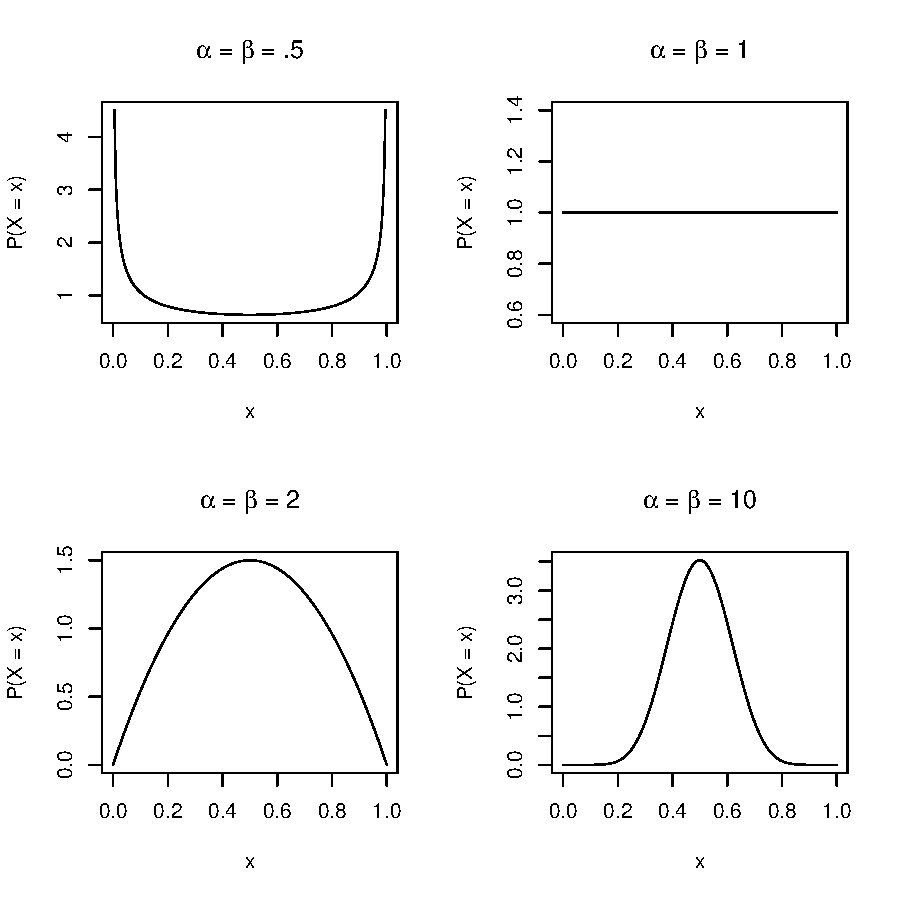
\includegraphics[width=\maxwidth]{figure/plot6-1} 

}



\end{knitrout}

\item
\item
\begin{enumerate}[label = (\alph*)]
\item
\item
\end{enumerate}
\item
\item 
\begin{enumerate}[label = (\alph*)]
\item
\item
\item
\item
\item
\item
\end{enumerate}
\item
\item
\item
\item 
\item
\item 
\begin{enumerate}[label = (\alph*)]
\item
\item
\item
\end{enumerate}
\item
\item 
\end{enumerate}
\newpage
\section*{R-Code}
\begin{verbatim}

## Require Packages
require(xtable)

x <- rep("NA", 8)
for (i in 1:8) x[i] <- choose(20, 21 - i)
x <- as.numeric(x)
sum(x) * (1/2)^20



\end{verbatim}
\end{document})
